\documentclass[11pt]{article}

\usepackage[a4paper,margin=1in]{geometry}
\usepackage{amsmath}
\usepackage{amssymb}
\usepackage{booktabs}
\usepackage{tabularx}
\usepackage{graphicx}
\usepackage[hidelinks]{hyperref}
\usepackage[authoryear,round]{natbib}
\usepackage{siunitx}
\usepackage{tikz}
\usepackage{colortbl}
\newcommand{\regimehead}[2]{%
  \noalign{\vskip 2pt}%
  \rowcolor{gray!18}\multicolumn{3}{@{}l@{}}{\rule{0pt}{2.4ex}\textbf{#1}\enspace\textnormal{\itshape#2}}\\[1pt]}
\usetikzlibrary{arrows.meta,positioning}
\sisetup{group-separator={,}, group-minimum-digits=4}

\title{Beyond Prevalence: Mitigation Signals and Interventions\\
for Histopathology Patch Classification and WSI-Level MIL}
\author{Yannik Queisler}
\date{\today}

\begin{document}
\maketitle

\begin{abstract}
\noindent A classifier can trail on a class for several distinct reasons, and mitigation methods differ in which of them they assume: some infer the need for mitigation from class frequency, others from example difficulty or from the sparsity of the observed feature support. This report is the thesis's authoritative reference for those mitigation methods and characterizes them along two orthogonal axes: the signal that identifies a class or example as needing mitigation---prevalence, independent evidence, difficulty, or coverage---and the level at which the intervention acts. Which methods apply depends on the input regime: labeled image patches support ordinary classification, whereas whole-slide image (WSI) diagnosis is commonly modeled as weakly supervised learning over patch-feature bags. Each method is therefore defined in the input form it consumes, with cross-entropy as the no-mitigation reference, and in enough mathematical detail to make its assumed mechanism, its tested adaptation, and its output semantics explicit.
\end{abstract}

\setcounter{tocdepth}{2}
\tableofcontents
\clearpage

\section{Introduction}
A pathology classifier can reach high aggregate accuracy while remaining unreliable on precisely the classes a diagnostic system is deployed to catch. When common tumor types dominate the training data, prevalence-sensitive evaluation rewards the classes that already dominate, so rare-class recall can degrade without the headline number moving. Long-tailed learning and medical-image evaluation literature therefore motivate classwise recall, macro F1, balanced accuracy, and calibration-aware probability metrics as primary outcomes in imbalanced settings \citep{saini2023tacklingClass,zhang2023deepLong,mosquera2024classImbalance}.

Imbalance methods often assume a specific prediction unit. Image-level methods use labeled images, image embeddings, or directly generated image samples, whereas WSI-level methods use weak labels over bags of instances together with attention, instance ranking, or bag-level representation learning. Each method family is therefore described in the input form it is designed to consume. The broader computational-pathology pipeline these regimes sit in---whole-slide imaging, patching into tiles, and weakly supervised multiple-instance learning over frozen foundation-model features---is introduced in the companion datasets report \citep{queisler2026datasets}.

Established mitigation methods differ not only in the level at which they intervene but also in the signal they use to infer which observations require mitigation. Class frequency is the signal most of the methods defined here consult, and a low class count conflates several distinct shortages: a small share relative to the other classes, a small absolute amount of independent evidence, intrinsic difficulty under the available representation, and poor coverage of the class's own variation. Section~\ref{sec:taxonomy} therefore makes both readings of the roster explicit, so that frequency is treated as a proxy for mitigation need rather than as its established cause. The methods themselves are drawn from the class-imbalance and long-tailed learning literature and are defined here in the order of their intervention level, stated in enough mathematical detail to make the assumed mechanism explicit. Two signals have no published representative, so two class-weighting rules are constructed here to complete the axis; both are marked as constructions of this thesis wherever they appear. The aim is otherwise not to propose new mitigation mechanisms, but to fix the method definitions, assumptions, and fidelity qualifications used when instantiating these methods on specific pathology datasets.

\paragraph{Prediction regimes.}
Two prediction regimes recur throughout this thesis. In the \emph{patch} regime, each labeled crop is an independent example: a frozen foundation-model encoder such as Virchow2 embeds the patch once, and a lightweight classifier head is trained on the resulting embedding \citep{zimmermann2024virchow2,vorontsov2024virchow}. In the \emph{WSI-bag} regime, a slide is represented as a bag of frozen patch-feature instances that share one weak slide-level label, and an attention-based MIL head aggregates the instances into a slide prediction. Both regimes consume embeddings from the same pathology foundation-model family but differ in supervision unit. Freezing the encoder isolates imbalance interventions from end-to-end backbone learning. Each non-baseline method exposes one imbalance-specific control, whose concrete search grid is an experimental decision rather than part of the method definition.

\section{Taxonomy}
\label{sec:taxonomy}
Two questions organize the tested methods. The first asks which signal a method consults to infer \emph{that} a class or an example needs help; the second asks at which level of the training pipeline it acts on that inference. The questions are independent, and neither answers the other: class-weighted CE gives example $i$ a weight $w_i=f(n_{y_i})$ that depends only on how many training examples share its class, while focal loss gives it a weight $w_i=f(p_{y_i})$ that depends only on how confidently the model already predicts its label, so two methods that are both loss reweighting can rest on entirely different assumptions about what causes tail failure. This section fixes the notation used throughout and then defines both axes.

\subsection{Notation}
Let $C$ be the number of target classes and let $n_c$ denote the number of training examples from class $c$, so that $N=\sum_{j=1}^{C}n_j$ is the training-set size and $\pi_c=n_c/N$ is the empirical prevalence of class $c$. For a labeled patch or slide-level bag with label $y\in\{1,\ldots,C\}$, the model outputs logits $\mathbf{z}\in\mathbb{R}^{C}$ and class probabilities
\begin{equation}
  p_c = \frac{\exp(z_c)}{\sum_{j=1}^{C}\exp(z_j)}.
  \label{eq:softmax}
\end{equation}
For WSI-bag methods, a slide is represented as a bag $B=\{\mathbf{x}_1,\ldots,\mathbf{x}_m\}$ of frozen patch-feature instances. The attention-MIL backbone maps each bag to a bag embedding $\mathbf{b}(B)$ and class logits. Unless a method explicitly changes the sampler, objective, or representation loss, the empirical class frequencies in the training set define the optimization signal.

\subsection{Intervention Levels}
\label{sec:intervention-axis}
The intervention axis records where in the learning problem a method acts. Cross-entropy (CE) is the no-mitigation reference condition on this axis: it uses the observed training distribution as given and does not rebalance samples, labels, costs, or representations. The remaining methods group as data-level sampling and augmentation, algorithm-level losses and prior corrections, hybrid sampling--loss methods, and representation or architecture-level methods \citep{saini2023tacklingClass,zhang2023deepLong}. Figure~\ref{fig:method-taxonomy} places the tested roster in these families, and Section~\ref{sec:methods} defines the methods in that order, since a shared intervention level implies shared machinery to describe.

\begin{figure}[ht]
  \centering
  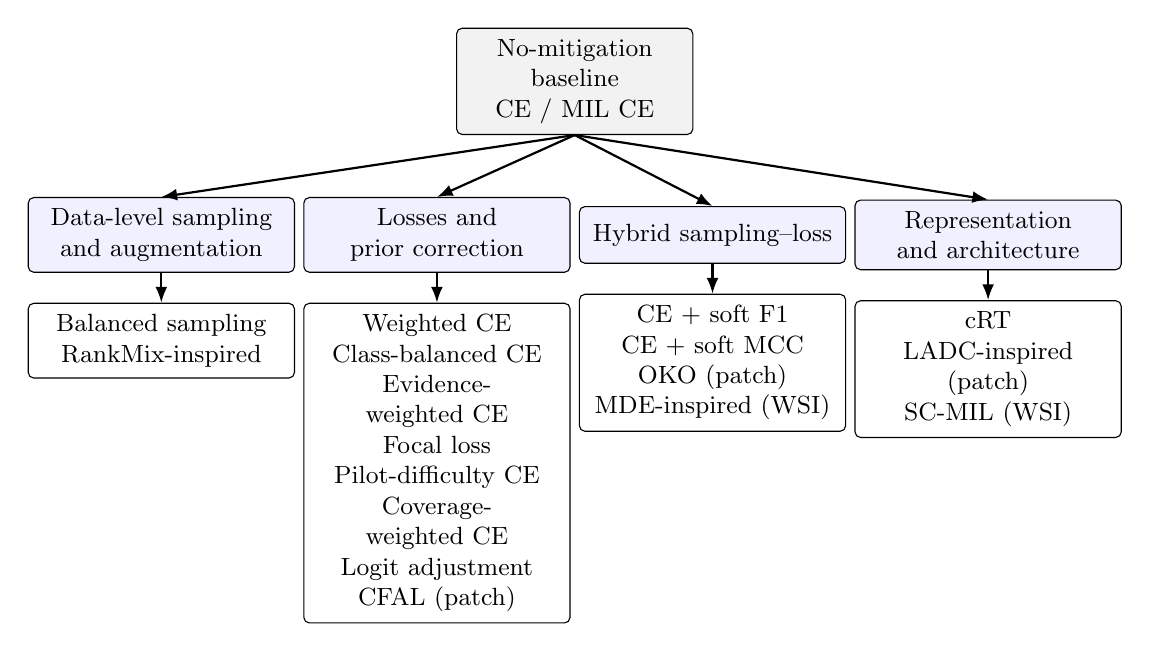
\begin{tikzpicture}[
    box/.style={draw, rounded corners=2pt, align=center, inner sep=4pt, font=\small, minimum height=0.72cm},
    baseline/.style={box, fill=gray!10, minimum width=3.0cm},
    family/.style={box, fill=blue!6, text width=3.1cm},
    method/.style={box, fill=white, text width=3.1cm},
    arrow/.style={-{Latex[length=2mm]}, thick}
  ]
    \node[baseline] (ce) at (0,0) {No-mitigation\\baseline\\CE / MIL CE};
    \node[family] (data) at (-5.25,-1.95) {Data-level sampling and augmentation};
    \node[method, below=0.38cm of data] (dataMethods) {Balanced sampling\\RankMix-inspired};
    \node[family] (loss) at (-1.75,-1.95) {Losses and prior correction};
    \node[method, below=0.38cm of loss] (lossMethods) {Weighted CE\\Class-balanced CE\\Evidence-weighted CE\\Focal loss\\Pilot-difficulty CE\\Coverage-weighted CE\\Logit adjustment\\CFAL (patch)};
    \node[family] (hybrid) at (1.75,-1.95) {Hybrid sampling--loss};
    \node[method, below=0.38cm of hybrid] (hybridMethods) {CE + soft F1\\CE + soft MCC\\OKO (patch)\\MDE-inspired (WSI)};
    \node[family] (repr) at (5.25,-1.95) {Representation and architecture};
    \node[method, below=0.38cm of repr] (reprMethods) {cRT\\LADC-inspired (patch)\\SC-MIL (WSI)};
    \draw[arrow] (ce.south) -- (data.north);
    \draw[arrow] (ce.south) -- (loss.north);
    \draw[arrow] (ce.south) -- (hybrid.north);
    \draw[arrow] (ce.south) -- (repr.north);
    \draw[arrow] (data) -- (dataMethods);
    \draw[arrow] (loss) -- (lossMethods);
    \draw[arrow] (hybrid) -- (hybridMethods);
    \draw[arrow] (repr) -- (reprMethods);
  \end{tikzpicture}
  \caption{Intervention-level organization of the tested methods. Cross-entropy is the no-mitigation reference; alternatives intervene through sampling, objectives, prior correction, feature mixing, feature synthesis, or representation and classifier design. Table~\ref{tab:signal-intervention} adds the orthogonal signal axis.}
  \label{fig:method-taxonomy}
\end{figure}

\subsection{Mitigation Signals}
\label{sec:signal-axis}
The signal axis records what a method must observe before it concludes that mitigation is warranted, stated as the quantity the method actually consults rather than the property it ultimately affects.

Four signals suffice to describe the tested roster (Table~\ref{tab:signals}). They are stated as properties of a class or example, independently of the intervention that acts on them.

\begin{table}[ht]
  \centering
  \footnotesize
  \begin{tabularx}{\linewidth}{@{}>{\raggedright\arraybackslash}p{0.15\linewidth}>{\raggedright\arraybackslash}p{0.44\linewidth}>{\raggedright\arraybackslash}X@{}}
    \toprule
    Signal & What it describes & Representative quantity \\
    \midrule
    Prevalence & Share of class $c$ relative to the remaining classes & $\pi_c$, support rank, imbalance ratio $\rho$ \\
    Evidence & Absolute amount of independent observation available for $c$ & Distinct patients, cases, or slides, effective support $N_{\mathrm{eff},c}$; $n_c$ read absolutely rather than as a share \\
    Difficulty & How hard a class or example is to classify under a fixed representation & Loss, predicted confidence $p_y$, decision margin, class difficulty $d_c$ \\
    Coverage & How well the observed examples span the within-class variation of $c$ & Manifold coverage $\mathrm{cov}_c$, effective rank of the class spectrum \\
    \bottomrule
  \end{tabularx}
  \caption{Signals a mitigation method can use to decide that a class or example needs help. Prevalence is relative and evidence is absolute; difficulty and coverage are properties of the data rather than of the class-size profile.}
  \label{tab:signals}
\end{table}

\subsubsection{Prevalence}
Prevalence is the share $\pi_c$ of class $c$ in the training distribution, together with the monotone summaries derived from it: the support rank of a class and the head-to-tail imbalance ratio $\rho=\max_c n_c/\min_c n_c$. It is a relative quantity. Rescaling every class count by a common factor leaves all prevalences unchanged, so a prevalence-aware rule behaves identically on a small and a large copy of the same class profile. This is the signal long-tailed learning has developed most thoroughly, and it underlies inverse-frequency weights, class-balanced samplers, and prior-corrected decision rules alike, all of which target a uniform posterior over classes rather than the observed one.

Prevalence is easily conflated with the amount of data a class actually carries, because both are usually read off the same counts $n_c$. The two come apart as soon as the profile changes shape rather than scale. Consider the training profiles $[8,8,8,8]$ and $[64,32,16,8]$. The scarcest class holds eight examples in both, so the material available for it is identical; its prevalence is $\tfrac{1}{4}$ in the first profile and $\tfrac{1}{15}$ in the second. A prevalence-aware rule treats that class very differently across the two profiles, whereas a rule driven by the absolute amount of evidence should treat it much the same. That absolute reading is the second signal.

\subsubsection{Independent Evidence}
Evidence is the absolute amount of independent observation available for a class, and in pathology it is not the raw example count. A patch is a training example, but patches drawn from one case are not independent observations of the class that case carries: they share its staining, scanner, preparation, and much of its morphology. Thousands of crops from a handful of participants therefore supply far less evidence than their number suggests, and the same holds inside a slide bag, whose instances share a single weak label. Evidence is consequently counted in \emph{split units}---the patients or cases over which partitions are drawn---together with the distinct slides beneath them. At WSI level the labelled slide is itself the independent unit, so a rare diagnosis represented by a few slides is evidence-poor however many instances those slides contain.

Unique unit counts are the primary measure, but they are coarse: two classes with the same number of cases can still differ in how interchangeable their patches are. \emph{Effective support} refines the count by discounting within-case redundancy. For class $c$, let $G_c$ be the number of split-unit or slide clusters contributing to it, let $m_{gc}$ be their sizes, and let $n_c=\sum_{g}m_{gc}$. Redundancy is summarized by the intraclass correlation (ICC) of a scalar per-example score, computed from the between-cluster and within-cluster mean squares $\mathrm{MS}_{B,c}$ and $\mathrm{MS}_{W,c}$ with the usual correction $m_{0,c}$ for unequal cluster sizes:
\begin{equation}
  m_{0,c}=\frac{n_c-\sum_{g=1}^{G_c}m_{gc}^2/n_c}{G_c-1},
  \qquad
  \operatorname{ICC}_c=
  \frac{\mathrm{MS}_{B,c}-\mathrm{MS}_{W,c}}
  {\mathrm{MS}_{B,c}+(m_{0,c}-1)\mathrm{MS}_{W,c}},
  \label{eq:icc}
\end{equation}
\noindent clipped to $[0,1]$. An ICC near zero means that examples from one case are no more alike than examples from different cases; an ICC near one means the case is effectively a single observation repeated. The corresponding effective support is
\begin{equation}
  N_{\mathrm{eff},c}=\frac{n_c}{1+(\overline m_c-1)\operatorname{ICC}_c},
  \label{eq:neff}
\end{equation}
\noindent where $\overline m_c$ is the mean cluster size. The two limits make the quantity readable: with $\operatorname{ICC}_c=0$ the class retains its full count $n_c$, and with $\operatorname{ICC}_c=1$ it collapses to $n_c/\overline m_c$, one observation per contributing case. Equations~\eqref{eq:icc}--\eqref{eq:neff} adjust a patch count for redundancy; they do not replace independent-unit counts, and the choice of per-example score, its cross-fitting, and the reference sets used to compute it are experimental decisions rather than part of the definition. A method is evidence-aware when a quantity of this kind---an independent-unit count or $N_{\mathrm{eff},c}$---enters its weights or its sampler, rather than the relative share $\pi_c$.

One distinction inside this signal matters for reading the roster, because two methods below weight classes by an \emph{effective number} that is not the quantity defined here. The class-balanced loss models diminishing returns as a function of the raw count alone through $E_c(\beta)$ in Equation~\eqref{eq:cb-effective-number}, and CFAL reuses the same construction. Both therefore read $n_c$ absolutely, which already separates them from the prevalence-driven methods, but neither asks how many independent units those examples came from: a class of \num{5000} patches drawn from four cases and one drawn from four hundred receive identical weights. Equation~\eqref{eq:neff} models the opposite quantity, redundancy-adjusted independent evidence, and is silent about diminishing returns. No published method reads it. The evidence channel is therefore supplied by a construction of this thesis, evidence-weighted CE (Section~\ref{sec:evi-ce}), which substitutes $N_{\mathrm{eff},c}$ for $n_c$ inside the power-law weight of class-weighted CE and so isolates the redundancy adjustment against an otherwise identical rule. Substituting $N_{\mathrm{eff},c}$ inside $E_c$ instead would combine both readings of the count, but the result is neither the established class-balanced loss nor a clean isolation of either mechanism, and it is retained only as a sensitivity analysis.

\subsubsection{Difficulty}
Difficulty is how hard a class or an example is to classify under a fixed representation, independently of how often it occurs. At example level it is read from the model's own state during training: the current loss, the predicted probability $p_y$ of the true class, or the margin between the true-class score and its strongest competitor. At class level it is measured as a probe error, for instance
\begin{equation}
  d_c = 1-\mathrm{recall}_c,
  \label{eq:difficulty}
\end{equation}
\noindent where $\mathrm{recall}_c$ is obtained from a class-balanced probe fitted on frozen features and evaluated out of fold, so that class size does not enter the score. A class whose morphology overlaps a neighbouring class is then difficult even when its support is ample, which is precisely what distinguishes this signal from the previous two. Two readings are worth separating. Intrinsic difficulty is a property of the representation and holds across training conditions; condition-specific learnability describes what remains recoverable from one particular training set and therefore moves with allocated support. Example-level and class-level difficulty are also not interchangeable: a loss-based weight adapts continuously during training and can chase label noise, whereas $d_c$ is estimated once and is stable but blind to which individual examples are hard.

\subsubsection{Coverage}
Coverage is how well the observed examples span the within-class variation of their class. A class can hold many independent cases and still cover its own distribution poorly, if those cases present one growth pattern, one grade, or one preparation while the population it is deployed on contains several. Coverage is therefore a property of the spread of a class in feature space rather than of any count, and it is the one signal the imbalance literature has left largely implicit. Stating it operationally requires a reference sample that stands for what the class actually looks like, since spanning is only defined relative to a target distribution. The natural, unmanipulated held-out cohort serves that role here.

Let $\{r_1,\ldots,r_{M_c}\}$ be the $M_c$ reference embeddings of class $c$ and $\{t_1,\ldots,t_{n_c}\}$ its $n_c$ observed training embeddings, both taken from the frozen encoder. Write $\mathrm{NND}_k(r_j)$ for the distance from $r_j$ to its $k$-th nearest neighbour among the remaining reference embeddings of the same class, which sets a local radius adapted to how densely the class populates that region; the neighbourhood size $k$ is fixed in advance. Coverage is the fraction of reference examples that have at least one training example inside their own neighbourhood,
\begin{equation}
  \mathrm{cov}_c=\frac{1}{M_c}\sum_{j=1}^{M_c}
  \mathbf{1}\Bigl[\exists\, i\in\{1,\ldots,n_c\}:\
  \lVert r_j-t_i\rVert<\mathrm{NND}_k(r_j)\Bigr].
  \label{eq:coverage}
\end{equation}
\begin{figure}[ht]
  \centering
  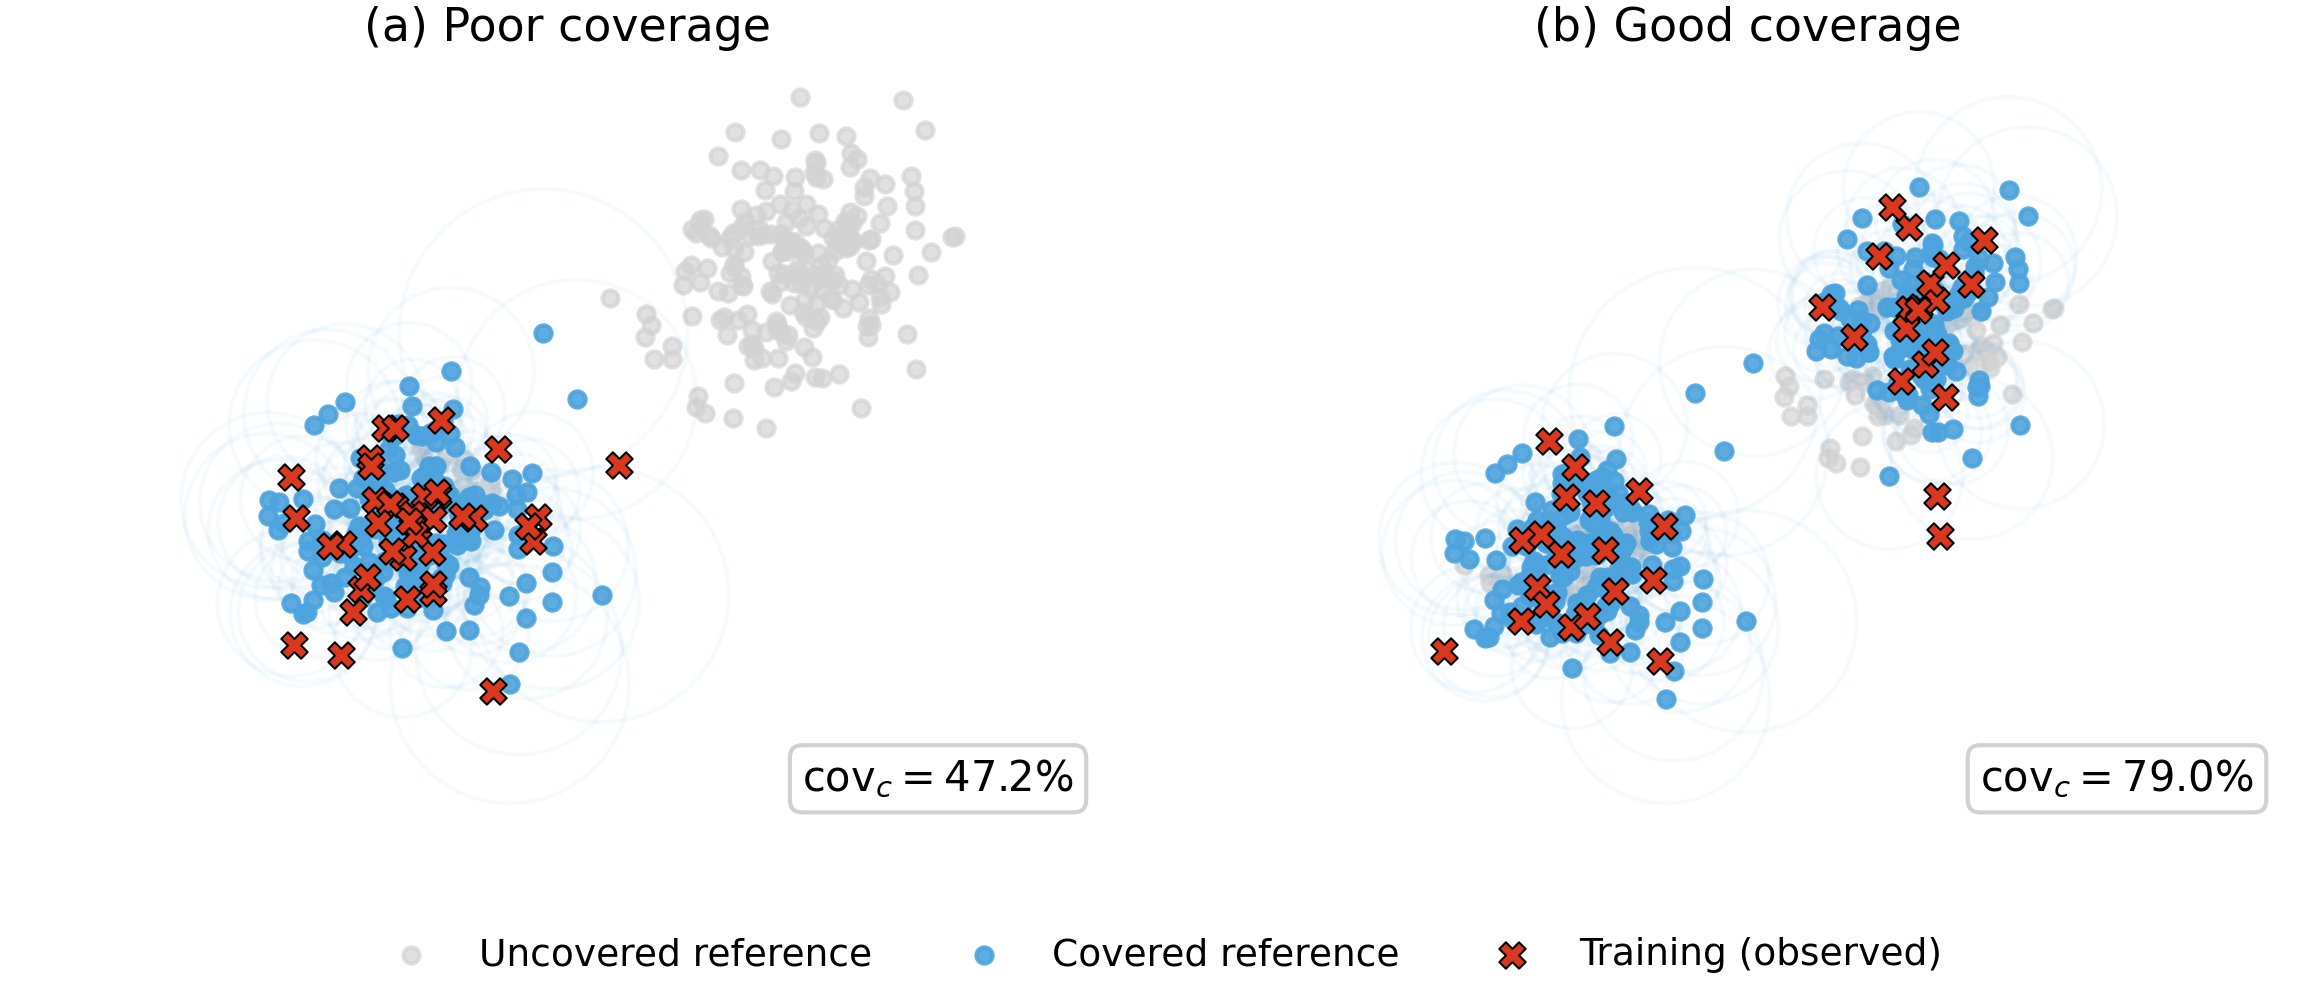
\includegraphics[width=\linewidth,keepaspectratio]{assets/coverage_plot.png}
  \caption{Coverage is not a count. Both panels show the same reference cloud, whose class has two morphological modes, and both training samples contain the same number of examples; the circles are the reference neighbourhoods of radius $\mathrm{NND}_k(r_j)$ that Equation~\eqref{eq:coverage} tests. In (a) the training material sits entirely in one mode, so the second mode stays unreached and half the class is uncovered. In (b) the same budget is spread across both modes and coverage rises accordingly. Prevalence and evidence are identical across the two panels, which is why coverage is a separate signal.}
  \label{fig:coverage}
\end{figure}

\noindent This is the manifold-coverage construction of \citet{naeem2020reliableFidelity}, which anchors the neighbourhood radii on the reference sample rather than on the observed one and is for that reason more robust to outlying training examples than the recall metric it refines \citep{kynkaanniemi2019improvedPrecision}. A region of the class that the training material never reaches lowers $\mathrm{cov}_c$ regardless of how many examples crowd the regions it does reach, which is exactly the failure mode a count cannot express and which Figure~\ref{fig:coverage} illustrates for a class with two morphological modes. Where no reference cohort is available, the covariance matrix of the class embeddings gives a reference-free substitute. Let $\lambda_1\geq\cdots\geq\lambda_D$ be its eigenvalues, each the variance of the class along one principal direction of the $D$-dimensional embedding space, and let $\widehat{\lambda}_i=\lambda_i/\sum_{j=1}^{D}\lambda_j$ be the same spectrum normalized to sum to one. With the Shannon entropy of that normalized spectrum,
\begin{equation}
  H(\widehat{\lambda})=-\sum_{i=1}^{D}\widehat{\lambda}_i\log\widehat{\lambda}_i,
  \qquad
  \mathrm{erank}_c=\exp\bigl(H(\widehat{\lambda})\bigr),
  \label{eq:effective-rank}
\end{equation}
\noindent the effective rank $\mathrm{erank}_c$ counts how many directions the class occupies: it equals one when all variance lies along a single direction and $D$ when the spectrum is flat \citep{roy2007effectiveRank}. The participation ratio $\bigl(\sum_i\lambda_i\bigr)^2/\sum_i\lambda_i^2$ summarizes the same spectrum with a different weighting. Either statistic detects collapse within the observed material but is silent about what was missed.

Two conditions keep Equation~\eqref{eq:coverage} from re-measuring a signal already defined above. Coverage estimated on more examples is mechanically larger, so classes must be compared at a matched sample size, by subsampling every class to the scarcest count and averaging over draws; otherwise the estimate tracks $n_c$ and reproduces prevalence or evidence under a different name. For the same reason the sampling unit must be the case rather than the patch, since several hundred crops of one biopsy occupy a single neighbourhood and would otherwise read as broad coverage. A further caution applies whenever training support is itself manipulated: subsampling a class changes which regions of it remain represented, so coverage of a constructed training manifest is partly an outcome of the allocation rather than a fixed property of the class. Read as a property of the class, it must be estimated on the eligible pool; read as a property of a training condition, it describes what that condition preserved. No published method consults either reading, which is why the coverage channel is supplied by a construction of this thesis, coverage-weighted CE (Section~\ref{sec:cov-ce}).

\subsubsection{Reading the Roster along Both Axes}
Signals are not to be confused with side effects. A method is treated as aware of a signal only when a quantity of that type enters its sampler, its objective, or its decision rule. Several methods reshape a property they never measure: RankMix-inspired mixing interpolates feature subsequences and thereby broadens coverage, SC-MIL compacts and separates bag embeddings, and the CFAL diversity regularizer spreads class prototypes apart. LADC-inspired feature calibration is the strongest instance of the same asymmetry, since repairing sparse tail support is its explicit purpose, yet it too is triggered by class support rather than by an estimate of what the class fails to span. None of them computes a coverage statistic and adapts its behaviour to it, which is what distinguishes them from coverage-weighted CE. Table~\ref{tab:signal-intervention} therefore records what each method consults alongside what it changes, and marks the difference between shaping a property and measuring it.

\begin{table}[!htbp]
  \centering
  \footnotesize
  \begin{tabularx}{\linewidth}{@{}>{\raggedright\arraybackslash}p{0.23\linewidth}>{\raggedright\arraybackslash}p{0.42\linewidth}>{\raggedright\arraybackslash}X@{}}
    \toprule
    Method & Mitigation signal & Intervention \\
    \midrule
    \regimehead{Both regimes}{patch and WSI-bag}
    CE, MIL CE & None; observed distribution used as given & None (reference) \\
    Balanced sampling & Prevalence, through $n_{y_i}^{-s}$ & Minibatch composition \\
    Weighted CE & Prevalence, through $n_c^{-s}$ & Per-example loss weight \\
    Logit adjustment & Prevalence, through $\widehat{\pi}_c$ explicitly & Logit and prior correction \\
    cRT & Prevalence, through balanced stage-two exposure & Classifier refit on a frozen representation \\
    Class-balanced CE & Absolute count with diminishing returns, through the effective number $E_c(\beta)$ & Per-example loss weight \\
    Focal loss & Difficulty, through the per-example confidence $p_y$ & Per-example loss weight \\
    Pilot-difficulty weighted CE & Difficulty, through the locked classwise probe score $d_c$ & Per-example class-dependent loss weight \\
    \regimehead{Patch regime}{only}
    Evidence-weighted CE & Independent evidence, through the redundancy-adjusted support $N_{\mathrm{eff},c}$ & Per-example class-dependent loss weight \\
    Coverage-weighted CE & Coverage, through the measured deficit $1-\mathrm{cov}_c$ & Per-example class-dependent loss weight \\
    CFAL & Absolute count, through the effective number $E_c$ of class $c$; difficulty, through $(1-a_{i,y_i})^{\gamma}$; shapes coverage without measuring it & Prototype head and margin objective \\
    LADC-inspired feature calibration & Tail-distribution sparsity and the feature statistics of neighbouring head classes; repairs coverage without measuring it & Calibrated feature synthesis and classifier refit on a frozen representation \\
    CE + soft F1 & Prevalence, through balanced sampling and equal classwise weight in the macro term & Sampler and auxiliary objective \\
    CE + soft MCC & Prevalence, through balanced sampling and the batch marginals $t_c,p_c$ & Sampler and auxiliary objective \\
    OKO & Prevalence, through uniform pair-class sampling & Set construction and set-aggregated loss \\
    \regimehead{WSI-bag regime}{only}
    RankMix-inspired & Difficulty, through teacher instance ranking; shapes coverage without measuring it & Bag-level feature augmentation \\
    SC-MIL & Label structure only; prevalence enters through class-aware batching; shapes coverage without measuring it & Contrastive term and CE curriculum \\
    MDE-inspired & Prevalence, through paired natural and balanced loaders & Dual experts and consistency term \\
    \bottomrule
  \end{tabularx}
  \caption{Each tested method read along both axes: the signal it consults to identify mitigation need, and the mechanism it changes to act on it, grouped by the prediction regime the method applies to. Methods sharing an intervention family can consult different signals, and methods sharing a signal can intervene at different levels. Method-specific symbols name the mechanism responsible and are defined with the method in Section~\ref{sec:methods}.}
  \label{tab:signal-intervention}
\end{table}

Read this way, the roster is anchored on one signal without being confined to it. Eight of the seventeen interventions consult prevalence alone, and SC-MIL adds a ninth partial case through class-aware batching. Difficulty is consulted at two different units: focal loss and the teacher ranking inside RankMix-inspired mixing score individual examples, while pilot-difficulty weighted CE scores whole classes from a locked balanced probe. Absolute count enters through the effective number of class-balanced CE and of CFAL, with CB-CE isolating that mechanism from the prototype head, margin objective, and affinity weighting that CFAL bundles with it. Independent evidence and coverage are each consulted by exactly one method, and both of those are constructions of this thesis rather than published baselines, since no established method reads either quantity; LADC-inspired calibration acts on coverage directly, by reconstructing tail feature support, but without measuring it.

Five interventions---class-weighted CE, class-balanced CE, evidence-weighted CE, pilot-difficulty weighted CE, and coverage-weighted CE---share a single intervention level and differ only in the per-class score they read, namely $n_c$, $E_c(\beta)$, $N_{\mathrm{eff},c}$, $d_c$, and $1-\mathrm{cov}_c$. All five apply a mean-one normalized class weight to unmodified CE, so the signal is the only quantity that varies across them.

This distribution determines where the roster can and cannot separate mechanisms. Contrasts among the prevalence-aware methods vary the intervention while holding the signal fixed; the five weighting rules vary the signal while holding the intervention fixed; and difficulty additionally admits a within-signal contrast between its example-level and class-level readings. The quantities defined above---$d_c$, $N_{\mathrm{eff},c}$, $\mathrm{cov}_c$, and their alignment with allocated support---are also carried forward as predictors in their own right, which examines each dimension independently of whether a method acting on it succeeds.

\section{Methods}
\label{sec:methods}
Each method is defined below in the input form it consumes, following the intervention families of Figure~\ref{fig:method-taxonomy}. The comparison is regime-specific. Patch methods consume frozen Virchow2 embeddings of controlled patches and optimize one shared MLP classifier head; CE-based patch methods use the same linear output layer, while CFAL replaces that layer with class prototypes and affinity-based prediction. WSI-bag methods consume complete eligible frozen-feature bags and optimize one shared attention-MIL head. Both regimes therefore rely on the same pathology foundation-model family, but they differ in supervision unit: one embedding per selected patch versus aggregation over every eligible instance on a slide, without bag truncation.

\subsection{Cross-Entropy Baseline}
Unweighted cross-entropy is the baseline because it is the standard supervised objective without an explicit class-imbalance correction. For an example with label $y$, the loss is
\begin{equation}
  \mathcal{L}_{\mathrm{CE}}(\mathbf{z},y) = -\log p_y.
  \label{eq:ce}
\end{equation}
In the patch regime, this objective trains the shared linear head on frozen Virchow2 patch embeddings from the controlled manifest. In the WSI-bag regime, the same objective trains the shared attention-MIL model on slide-level feature bags. In both cases, CE uses the observed class distribution directly: majority classes appear more often in minibatches and therefore contribute more loss terms over an epoch. This makes CE an appropriate reference for asking whether an imbalance-specific intervention actually improves the rare-class tradeoff.

\subsection{Data-Level Sampling and Augmentation}
Data-level methods change what the optimizer sees, rather than changing the mathematical penalty assigned to one observed example. In the taxonomy, this family includes resampling, augmentation, and WSI-specific feature mixing strategies that make minority or informative examples more visible during training \citep{saini2023tacklingClass}.

\subsubsection{Balanced Sampling}
Balanced sampling changes minibatch composition by sampling training examples with probabilities related to their class support through a strength $s\in[0,1]$. For an example $i$ with class $y_i$, the sampler weight is proportional to
\begin{equation}
  q_i(s) \propto n_{y_i}^{-s}.
  \label{eq:balanced-sampling}
\end{equation}
After normalization across the training set, $s=0$ recovers ordinary sampling and $s=1$ gives equal expected exposure to every class; intermediate values partially rebalance the data. The patch variant applies this sampler to patch examples and still optimizes CE. The MIL variant applies the same idea at slide-bag level and also optimizes CE. Balanced sampling therefore tests a pure data-level intervention without changing the loss formula.

\subsubsection{RankMix-Inspired Feature Mixing}
RankMix is a WSI-native data-augmentation method for weakly supervised slide classification. Ordinary image mixup assumes two inputs with compatible spatial shapes, but WSI bags can contain different numbers of feature instances and lack instance-level labels. RankMix addresses this by mixing representative feature subsequences rather than raw slides \citep{chen2023rankmix}. The tested variant is called \emph{RankMix-inspired} because it preserves the source method's teacher ranking, representative subsequence selection, feature interpolation, mixed labels, and reinitialized student, but does not reproduce the paper's complete combination of instance-max and bag-level objectives. Its student instead uses soft-label CE on the mixed bag prediction. Results therefore test this specified adaptation, not a faithful reproduction of the full source method.

The tested implementation follows the defining two-stage teacher--student procedure. First, a teacher attention-MIL model is trained with slide labels for exactly the protocol-defined budget $U$ of optimizer updates, using the same MIL architecture and optimization settings as plain MIL CE. For each bag $B=\{\mathbf{x}_1,\ldots,\mathbf{x}_m\}$ and target class, the teacher assigns ranking scores to instances using its softmax probability for that class; the top-$k$ instances are kept as a representative subsequence, where $k=\min(|B_a|,|B_b|)$ for the two bags being mixed, and their original within-bag order is preserved after selection. The student MIL model is then reinitialized and receives its own $U$ updates on bags built from these ranked subsequences.

Mixing itself follows the mixup idea in feature space. For two bags $a$ and $b$, let $H_a$ and $H_b$ denote the selected instance-feature matrices and $\mathbf{y}_a,\mathbf{y}_b$ the corresponding one-hot slide labels. A scalar mixing coefficient $\lambda\in(0,1)$ controls how much of each bag is retained:
\begin{equation}
  \widetilde{H}=\lambda H_a+(1-\lambda)H_b,
  \qquad
  \widetilde{\mathbf{y}}=\lambda \mathbf{y}_a+(1-\lambda)\mathbf{y}_b.
  \label{eq:rankmix}
\end{equation}
\noindent When $\lambda$ is close to one, the mixed bag resembles bag $a$; when it is close to zero, it resembles bag $b$. Values near $\lambda=\tfrac{1}{2}$ interpolate more evenly between the two sources. RankMix does not fix $\lambda$ to a single value. Instead, each mixed example draws
\begin{equation}
  \lambda \sim \mathrm{Beta}(\alpha,\alpha),
  \label{eq:rankmix-beta}
\end{equation}
\noindent independently. The Beta distribution is a standard choice on the open interval $(0,1)$ because it is flexible and symmetric when both shape parameters are equal. With density
\begin{equation}
  f(\lambda;\alpha,\alpha)\propto \lambda^{\alpha-1}(1-\lambda)^{\alpha-1},
  \qquad \lambda\in(0,1),
  \label{eq:beta-density}
\end{equation}
\noindent the parameter $\alpha>0$ controls how strongly mixing concentrates around the endpoints versus the center. For $\alpha=1$, $\mathrm{Beta}(1,1)$ is uniform on $(0,1)$. Larger $\alpha$ pushes $\lambda$ toward $\tfrac{1}{2}$; smaller $\alpha$ keeps mixtures closer to one source bag. The reference default is $\alpha=\num{1.0}$, and $\alpha$ is selected on validation. The student is trained with soft-label CE on the mixed bags and labels $\widetilde{\mathbf{y}}$. This is a data-level feature-space augmentation while retaining the common attention-MIL prediction architecture.

\subsection{Algorithm-Level Losses}
Algorithm-level methods keep the training examples fixed but alter how errors are penalized. They are cost-sensitive or difficulty-sensitive objectives: minority examples may receive larger explicit weights, or easy examples may contribute less to the gradient \citep{saini2023tacklingClass,scholz2024imbalanceAware}.

\subsubsection{Class-Weighted Cross-Entropy}
Class-weighted CE multiplies each example's CE term by a class-dependent cost controlled by the same strength $s\in[0,1]$:
\begin{equation}
  \mathcal{L}_{\mathrm{WCE}}(\mathbf{z},y) = -w_y\log p_y,
  \qquad
  w_c(s) \propto n_c^{-s}.
  \label{eq:weighted-ce}
\end{equation}
The implementation normalizes these weights so that their mean across classes is one. Here $s=0$ recovers unweighted CE and $s=1$ gives inverse-frequency weighting; intermediate values reduce the correction. This method leaves the sample order and model architecture unchanged, but increases the loss contribution of classes with fewer training examples. It is evaluated for both patch classification and attention-MIL.

\subsubsection{Class-Balanced Cross-Entropy by Effective Number}
\label{sec:cb-ce}
Class-balanced (CB) cross-entropy replaces inverse-frequency weighting by a saturating notion of how much a class count is worth \citep{cui2019classBalanced}. Its premise is that additional examples of a class need not contribute linearly increasing information: as support grows, examples increasingly resemble ones already seen, so the marginal contribution of the next example diminishes. For class $c$ with training count $n_c$, the effective number of samples is
\begin{equation}
  E_c(\beta)=\frac{1-\beta^{n_c}}{1-\beta},
  \qquad 0\leq\beta<1,
  \label{eq:cb-effective-number}
\end{equation}
\noindent and the class weight is proportional to its inverse. As for class-weighted CE, the implementation normalizes the weights to mean one across classes,
\begin{equation}
  w_c^{\mathrm{CB}}(\beta)=
  \frac{\widetilde w_c^{\mathrm{CB}}(\beta)}
       {\frac{1}{C}\sum_{j=1}^{C}\widetilde w_j^{\mathrm{CB}}(\beta)},
  \qquad
  \widetilde w_c^{\mathrm{CB}}(\beta)=\frac{1-\beta}{1-\beta^{n_c}},
  \label{eq:cb-weight}
\end{equation}
\noindent and optimizes
\begin{equation}
  \mathcal{L}_{\mathrm{CB}}(\mathbf z,y;\beta)=-w_y^{\mathrm{CB}}(\beta)\log p_y.
  \label{eq:cb-ce}
\end{equation}
\noindent The single control $\beta$ sets the count scale at which those diminishing returns take effect. At $\beta=0$ every effective number equals one and the objective reduces to ordinary CE; as $\beta\rightarrow1$ the normalized weights approach inverse-count weighting. Intermediate values are the informative ones, because they separate a \emph{saturating} count correction from the power-law correction $n_c^{-s}$ of Equation~\eqref{eq:weighted-ce}: under the power law every doubling of class support changes the weight by the same factor, whereas under Equation~\eqref{eq:cb-weight} the weight stops responding once $n_c$ exceeds roughly $(1-\beta)^{-1}$. The reference default is $\beta=\num{0.999}$; $\beta$ is the imbalance control selected on validation.

Two properties make this method the cleanest available isolation of the effective-number mechanism. First, $n_c$ enters absolutely rather than as a share, so unlike the prevalence-driven methods the weights change when a class profile is scaled rather than reshaped. Here $n_c$ is the prediction-unit count of the training condition: labeled patches for patch classification and labeled slides for WSI-level MIL. Second, CB-CE changes neither the sampler, the head geometry, nor the output semantics, while CFAL couples the same effective number to class prototypes, a margin objective, an affinity-based difficulty factor, and a diversity regularizer (Equation~\eqref{eq:cfal-total}). An effect of CFAL therefore cannot be attributed to its effective-number term alone, whereas an effect of CB-CE can. The method is evaluated in both regimes.

\subsubsection{Evidence-Weighted Cross-Entropy}
\label{sec:evi-ce}
No published mitigation method weights classes by the number of independent observations behind them. Class-weighted CE and class-balanced CE both read the raw example count $n_c$, which in pathology overstates what a class carries: patches drawn from one case share its staining, scanner, preparation, and much of its morphology (Section~\ref{sec:signal-axis}). Evidence-weighted CE is constructed for this thesis to supply that missing signal channel and is reported as a thesis construction rather than as a published baseline.

The rule keeps the functional form of Equation~\eqref{eq:weighted-ce} and changes only the support measure it reads. With the redundancy-adjusted effective support $N_{\mathrm{eff},c}$ of Equation~\eqref{eq:neff} and the mean-one normalization used by the other weighting methods,
\begin{equation}
  w_c^{\mathrm{EVI}}(\tau)=
  \frac{N_{\mathrm{eff},c}^{-\tau}}
       {\frac{1}{C}\sum_{j=1}^{C}N_{\mathrm{eff},j}^{-\tau}},
  \qquad
  \mathcal{L}_{\mathrm{EVI}}(\mathbf z,y;\tau)=-w_y^{\mathrm{EVI}}(\tau)\log p_y.
  \label{eq:evi-ce}
\end{equation}
\noindent The exponent $\tau\geq0$ is the single imbalance control, and $\tau=0$ recovers ordinary CE. Because Equation~\eqref{eq:evi-ce} differs from class-weighted CE only in substituting $N_{\mathrm{eff},c}$ for $n_c$, a difference between the two is attributable to the redundancy adjustment alone: the two rules coincide when every class draws its examples from equally many independent units and diverge exactly when a class's examples concentrate in few cases. Both remain power-law corrections, which separates this method in turn from the saturating count correction of Section~\ref{sec:cb-ce}.

Two properties of the signal carry into the method. Effective support is a property of the training condition rather than of the class, so it is recomputed for each condition exactly as $n_c$ is. Its intraclass correlation requires a per-example scalar score whose choice, cross-fitting, and reference sets are experimental decisions rather than part of the definition, so the weights inherit an estimation error that class-weighted CE does not carry. The method is evaluated in the patch regime only: at WSI level the labelled slide is already the independent unit, so $\overline m_c=1$, $N_{\mathrm{eff},c}=n_c$, and the objective collapses onto class-weighted CE.

\subsubsection{Focal Loss}
Focal loss reduces the contribution of confidently classified examples and concentrates optimization on examples that remain difficult. With focusing parameter $\gamma$, the multiclass focal objective is
\begin{equation}
  \mathcal{L}_{\mathrm{focal}}(\mathbf{z},y) =
  -(1-p_y)^{\gamma}\log p_y.
  \label{eq:focal}
\end{equation}
The reference default is $\gamma=\num{2.0}$ for both regimes; $\gamma$ is the imbalance control selected on validation while the rest of the training protocol is held fixed. The method is relevant to imbalance because many minority-class examples can remain hard under a classifier dominated by head-class gradients, but the focal term does not directly encode the class counts. It is therefore a difficulty-sensitive loss rather than a sampler or explicit prior correction.

\subsubsection{Pilot-Difficulty Weighted Cross-Entropy}
\label{sec:pdw-ce}
Class-difficulty based weighting (CDB-W) replaces class frequency by measured classwise prediction difficulty as the signal for cost-sensitive learning \citep{sinha2022classDifficulty}. It separates the assumption that a class is difficult because it is rare from the possibility that a comparatively frequent class remains intrinsically difficult under the available representation. In the source method, difficulty after epoch $e$ is
\begin{equation}
  d_{c,e}=1-A_{c,e},
  \label{eq:cdb-difficulty}
\end{equation}
\noindent where $A_{c,e}$ is classwise accuracy on a separate balanced monitor set, and examples of class $c$ receive the weight $d_{c,e}^{\tau_e}$, so that the objective at epoch $e$ uses the difficulties measured at $e-1$. The source additionally schedules the exponent $\tau_e$ from the imbalance of classwise performance, which makes CDB-W a dynamic class-difficulty method rather than a count-based reweighting rule. The mechanism differs from focal loss in the unit it describes: focal loss asks whether \emph{this example} is currently hard through $p_y$, whereas CDB-W asks whether \emph{this class} is currently hard. A frequent but morphologically ambiguous class can therefore be upweighted above a rare but already separable one.

\paragraph{Thesis adaptation.}
A source-faithful implementation requires a balanced monitor set that is re-evaluated throughout training. The natural-validation cohort is the only held-out data of that kind, and it is reserved for hyperparameter and checkpoint selection; feeding it back as a per-epoch training signal would dissolve the separation between training and model selection. The tested variant therefore uses the class difficulty $d_c$ of Equation~\eqref{eq:difficulty}, obtained once from the class-balanced out-of-fold probe and locked before the training conditions are constructed. With a fixed $\epsilon>0$ that only prevents zero weights for a perfectly separated class, the mean-one normalized weight is
\begin{equation}
  w_c^{\mathrm{PDW}}(\tau)=
  \frac{(d_c+\epsilon)^{\tau}}
       {\frac{1}{C}\sum_{j=1}^{C}(d_j+\epsilon)^{\tau}},
  \label{eq:pdw-weight}
\end{equation}
\noindent and the objective is
\begin{equation}
  \mathcal{L}_{\mathrm{PDW}}(\mathbf z,y;\tau)=-w_y^{\mathrm{PDW}}(\tau)\log p_y.
  \label{eq:pdw-ce}
\end{equation}
\noindent The exponent $\tau\geq0$ is the single imbalance control: $\tau=0$ recovers ordinary CE, and larger values concentrate loss weight on the classes the balanced probe found hardest. Because this variant fixes difficulty in advance instead of tracking it during training, it is reported as \emph{pilot-difficulty weighted CE (CDB-W-inspired)} rather than as a reproduction of CDB-W. It is not a dynamic method: it cannot react to a class whose difficulty changes as training proceeds, and it inherits whatever estimation error the probe carries.

That static reading is nevertheless the more informative one for a controlled comparison. Because $d_c$ is estimated on a balanced reference before support is allocated, it stays fixed while the training conditions vary which classes are placed in the tail. Under a difficulty-aligned assignment the scarce classes are also the hard ones, so difficulty weighting and frequency weighting favor the same classes; under a difficulty-reversed assignment they issue opposite instructions. The contrast between this method and class-weighted CE therefore separates whether a class benefits from mitigation because it is rare or because it is hard, which a difficulty score re-estimated inside each condition would confound. The method leaves the sampler and architecture unchanged and is evaluated in both regimes.

\subsubsection{Coverage-Weighted Cross-Entropy}
\label{sec:cov-ce}
Coverage is the signal of Section~\ref{sec:signal-axis} that no published mitigation method consults, even though several methods reshape it. Coverage-weighted CE is constructed for this thesis to close that channel and is likewise reported as a thesis construction rather than as a published baseline. It asks whether upweighting the classes whose observed material spans their own variation poorly differs from upweighting the classes that are merely small.

The construction follows pilot-difficulty weighted CE and substitutes the coverage deficit for the probe error. With $\mathrm{cov}_c$ from Equation~\eqref{eq:coverage} and a fixed $\epsilon>0$ that only prevents a zero weight for a fully covered class,
\begin{equation}
  w_c^{\mathrm{COV}}(\tau)=
  \frac{(1-\mathrm{cov}_c+\epsilon)^{\tau}}
       {\frac{1}{C}\sum_{j=1}^{C}(1-\mathrm{cov}_j+\epsilon)^{\tau}},
  \qquad
  \mathcal{L}_{\mathrm{COV}}(\mathbf z,y;\tau)=-w_y^{\mathrm{COV}}(\tau)\log p_y.
  \label{eq:cov-ce}
\end{equation}
\noindent The exponent $\tau\geq0$ is again the single imbalance control, with $\tau=0$ recovering ordinary CE.

Which reading of coverage enters the weight is a design decision rather than a detail. Estimated on the eligible pool, $\mathrm{cov}_c$ is a fixed property of the class and behaves like $d_c$: locked before the training conditions are constructed and constant across them. Estimated on the training manifest of one condition, it describes what that condition preserved and therefore moves with the allocation, as $n_c$ does. The tested variant uses the condition reading, because the deficit the weights are meant to answer is the one the allocated material actually leaves open; the pool reading is retained as a sensitivity analysis. Under either reading the estimate is taken at matched sample size with case-level subsampling, without which the score tracks class size and the method silently reduces to a count-based rule.

The method is evaluated in the patch regime only, since a rare diagnosis contributes too few bag embeddings for Equation~\eqref{eq:coverage} to be estimated against a reference cohort at WSI level. It is the only intervention in the roster whose weights respond to a coverage statistic: LADC-inspired feature synthesis repairs coverage but is triggered by class support, so the contrast between them separates measuring the deficit from reconstructing it.

\subsubsection{Logit Adjustment}
Logit adjustment explicitly corrects for the empirical training prior \citep{menon2021longTail}. Let
\begin{equation}
  \widehat{\pi}_c=\frac{n_c}{\sum_{j=1}^{C}n_j}
  \label{eq:empirical-prior}
\end{equation}
denote the class prior estimated only from the current training condition. The control $\tau\geq0$ determines the strength of the correction; $\tau=0$ recovers ordinary CE. In the train-time form, adjusted logits are used inside the loss,
\begin{equation}
  \mathcal{L}_{\mathrm{LA-train}}(\mathbf z,y)
  =-\log\frac{\exp(z_y+\tau\log\widehat{\pi}_y)}
  {\sum_{c=1}^{C}\exp(z_c+\tau\log\widehat{\pi}_c)}.
  \label{eq:logit-adjustment-train}
\end{equation}
The positive prior term makes head classes harder to fit during training, inducing a classifier whose unadjusted logits favor a class-balanced target. In the post-hoc form, a model is trained with ordinary CE and corrected only at inference,
\begin{equation}
  p_c^{\mathrm{LA}}(\mathbf x)=
  \frac{\exp(z_c(\mathbf x)-\tau\log\widehat{\pi}_c)}
  {\sum_{j=1}^{C}\exp(z_j(\mathbf x)-\tau\log\widehat{\pi}_j)}.
  \label{eq:logit-adjustment-posthoc}
\end{equation}
The sign difference follows from where the correction is applied: the train-time loss learns against prior-shifted logits, whereas the post-hoc rule removes the observed training prior from ordinary CE logits. Both patch and WSI regimes use the same definition at their respective prediction unit. Because either form deliberately changes the implied target prior, its probabilities should not be interpreted as calibrated for the natural test prevalence without an explicit target-prior assumption. Discrimination and calibration are therefore reported together, with post-hoc temperature scaling kept conceptually separate from prior correction.

Score variants with different interpretations are retained as separate outputs. For an ordinary CE score $z_c^{\mathrm{CE}}$, post-hoc logit adjustment uses $z_c^{\mathrm{CE}}-\tau\log\widehat\pi_c$ for class-balanced decisions; this score is not reported as a probability calibrated to the natural target prevalence. Under the prior-shift assumption, probabilities for a target prior $\pi_c^{\mathrm{target}}$ instead normalize the logits
\begin{equation}
  z_c^{\mathrm{CE}}-\log\widehat\pi_c+\log\pi_c^{\mathrm{target}}.
  \label{eq:posthoc-target-prior}
\end{equation}
\noindent For train-time adjustment, CE is applied to $g_c=z_c+\tau\log\widehat\pi_c$. Because $g_c$ approximates training-posterior logits, the corresponding target-prevalence logits are
\begin{equation}
  z_c+(\tau-1)\log\widehat\pi_c+\log\pi_c^{\mathrm{target}}.
  \label{eq:train-time-target-prior}
\end{equation}
\noindent The unadjusted $z_c$ is the train-time method's validation-selected discrimination score but is fully prior-stripped only when $\tau=1$. The target prior is estimated separately on each natural-validation split and applied only to the corresponding test split. Temperature scaling is fitted on natural-validation NLL after the applicable target-prior correction and then applied unchanged to test logits. Raw, balanced-decision, target-prior-corrected, and temperature-scaled outputs remain separate; a single temperature corrects overall sharpness rather than class-specific prior mismatch.

Balanced Softmax is closely related prior-correction literature: it modifies the softmax denominator using class frequencies and motivates the same distinction between representation learning under a long-tailed source and decision rules for a balanced target \citep{ren2020balancedMeta}. It is not an additional tested method; it is included to situate logit adjustment among count-aware softmax objectives.

\subsubsection{Center-Focused Affinity Loss (CFAL)}
Center-focused affinity loss (CFAL) replaces the linear softmax head with learnable class prototypes and an affinity-based training objective \citep{mahbub2024centerFocused}. The motivation is that minority histology classes can remain visually similar in embedding space even when a frozen encoder already separates them coarsely; pulling examples toward compact class centers and penalizing confusion with nearby wrong-class prototypes can therefore improve tail-class boundaries without changing the sampler.

The tested patch implementation keeps the shared MLP trunk that maps a frozen Virchow2 embedding $\mathbf{x}$ to a hidden representation $\mathbf{z}=f(\mathbf{x})\in\mathbb{R}^{512}$, but replaces the final linear map with one learnable prototype $\mathbf{w}_c\in\mathbb{R}^{512}$ per class. Both embeddings and prototypes are L2-normalized before affinity computation. The Gaussian affinity between example $i$ and class $c$ is
\begin{equation}
  a_{ic}=\exp\!\left(-\frac{\|\hat{\mathbf{z}}_i-\hat{\mathbf{w}}_c\|_2^2}{\sigma}\right),
  \qquad
  \hat{\mathbf{v}}=\frac{\mathbf{v}}{\|\mathbf{v}\|_2},
  \label{eq:cfal-affinity}
\end{equation}
\noindent where $\sigma$ controls how quickly affinity decays with prototype distance. At inference, class scores are $\log a_{ic}$ followed by softmax normalization. The affinities $a_{ic}\in(0,1]$ are geometric similarity scores, not class probabilities: they are trained with a margin objective and never optimized to satisfy likelihood or calibration constraints. Applying softmax to $\log a_{ic}$ therefore yields a convenient ranking score for argmax decisions, but it should not be read as a calibrated estimate of $P(y=c\mid \mathbf{x})$ without additional post-hoc mapping.

Training optimizes a margin term on affinities rather than cross-entropy on logits. For batch index $i$ with label $y_i$, define the per-example margin loss
\begin{equation}
  \ell_i=\sum_{c\ne y_i}\max\bigl(0,\, \lambda + a_{ic}-a_{i,y_i}\bigr),
  \label{eq:cfal-margin}
\end{equation}
\noindent which penalizes wrong-class affinities that exceed the true-class affinity by less than margin $\lambda$. A diversity regularizer $R(\mathbf{W})$ encourages prototypes to spread apart by penalizing deviations of pairwise squared distances from their mean. The total objective combines class reweighting, a center-focused local weight, and prototype diversity:
\begin{equation}
  \mathcal{L}_{\mathrm{CFAL}}=
  \frac{1}{B}\sum_{i=1}^{B}
  \frac{1}{E_{y_i}}
  (1-a_{i,y_i})^{\gamma}\,\ell_i
  + R(\mathbf{W}),
  \label{eq:cfal-total}
\end{equation}
\noindent where $E_c$ is the effective number of training examples in class $c$ derived from class count $n_c$ and hyperparameter $\beta$, and $\gamma$ up-weights examples whose true-class affinity remains low. Unlike the CE plus soft-F1 and soft-MCC hybrids, CFAL does not use balanced oversampling: it is categorized as an algorithm-level patch method because it changes the head and loss while keeping the natural training distribution.

The reference defaults are $\lambda=\num{0.1}$, $\beta=\num{0.999}$, and $\gamma=\num{2.0}$ following Mahbub et al.; all three are held fixed and the affinity bandwidth $\sigma$ is the imbalance control selected on validation. The paper's $\sigma=\num{130}$ was calibrated for un-normalized AlexNet FC features; on L2-normalized \num{2560}-dimensional Virchow2 vectors that scale is far too large and collapses all pairwise affinities, so the tested implementation evaluates a range matched to the normalized embedding geometry. CFAL is evaluated only in the patch regime because the source method assumes instance-level labels rather than weak slide-level bags.

\subsection{Hybrid Sampling--Loss Methods}
Hybrid methods combine data-level and algorithm-level changes. The Scholz-style patch objectives below adapt the metric-derived losses of Scholz et al.\ for imbalanced medical classification \citep{scholz2024imbalanceAware}. Both tested variants use class-balanced oversampling together with metric-derived losses, so their effect cannot be attributed only to a new loss or only to a new sampler.

\subsubsection{Scholz-Style CE + Soft F1}
The intuition is that CE optimizes the log-probability of the correct class one example at a time, whereas macro F1 evaluates a different object: the balance between precision and recall at class level. Under class imbalance, this distinction matters because a model can reduce CE substantially by fitting frequent classes while still leaving tail-class recall or precision weak.

The obstacle is that ordinary F1 is computed from hard counts after prediction, so it is not directly usable as a gradient-based training loss. The Scholz-style soft-F1 objective replaces those hard counts with probability-weighted counts inside each minibatch. For one class, a confident correct prediction contributes almost one soft true positive, a confident prediction for the wrong class contributes to soft false positives, and low probability on a true class contributes to soft false negatives. Formally, for one-hot labels $y_i$ and predicted probabilities $\hat{y}_i$:
\begin{equation}
  \mathrm{TP}=\sum_i y_i\hat{y}_i,\quad
  \mathrm{FP}=\sum_i (1-y_i)\hat{y}_i,\quad
  \mathrm{FN}=\sum_i y_i(1-\hat{y}_i).
  \label{eq:soft-confusion-f1}
\end{equation}
\noindent These terms keep the familiar meaning of a confusion matrix but make every component differentiable with respect to the model probabilities. They then define soft precision, soft recall, and soft F1:
\begin{equation}
  \mathrm{F1}_{\mathrm{soft}} =
  \frac{2\,\mathrm{precision}_{\mathrm{soft}}\,\mathrm{recall}_{\mathrm{soft}}}
       {\mathrm{precision}_{\mathrm{soft}}+\mathrm{recall}_{\mathrm{soft}}}.
  \label{eq:soft-f1}
\end{equation}
\noindent The multiclass implementation applies this construction separately to each class and averages the resulting classwise terms. This macro-style averaging is the imbalance-aware part: each class contributes one term regardless of how many samples it has in the full dataset. The tested objective does not replace CE completely; it adds the metric-derived term to CE so that optimization still rewards calibrated class probabilities while also pushing the minibatch toward higher macro soft F1:
\begin{equation}
  \mathcal{L}_{\mathrm{CE+F1}} = \mathcal{L}_{\mathrm{CE}} +
  \lambda_{\mathrm{aux}}
  \left(1-\frac{1}{C}\sum_{c=1}^{C}\mathrm{F1}_{\mathrm{soft},c}\right).
  \label{eq:ce-soft-f1}
\end{equation}
\noindent The auxiliary weight $\lambda_{\mathrm{aux}}>0$ controls the contribution of the soft-F1 term and is selected on validation. This loss is trained with balanced sampling on the patch manifest. That design is important for interpretation: the loss tries to optimize a macro-style class metric, while the sampler ensures that tail classes occur often enough in minibatches for their soft-F1 terms to provide a regular training signal.

\subsubsection{Scholz-Style CE + Soft MCC}
The soft-MCC variant uses the same principle as soft F1---replace hard evaluation counts with differentiable probability masses---but starts from the Matthews correlation coefficient (MCC). Whereas F1 for one class depends mainly on that class's positive predictions, MCC is built from the full confusion matrix and therefore reacts to false positives, false negatives, and true negatives at the same time. In binary problems it is often preferred in imbalanced settings because it can remain informative when one class dominates the dataset: accuracy can look high while predictions are still systematically biased, but MCC penalizes both kinds of mistakes jointly.

\paragraph{Binary MCC as a correlation coefficient.}
For one class treated as positive, write TP, TN, FP, and FN for the four confusion-matrix cells. The standard MCC is
\begin{equation}
  \mathrm{MCC} =
  \frac{\mathrm{TP}\cdot\mathrm{TN}-\mathrm{FP}\cdot\mathrm{FN}}
       {\sqrt{(\mathrm{TP}+\mathrm{FP})(\mathrm{TP}+\mathrm{FN})
              (\mathrm{TN}+\mathrm{FP})(\mathrm{TN}+\mathrm{FN})}}.
  \label{eq:binary-mcc}
\end{equation}
\noindent The numerator compares co-occurrence of correct positive and correct negative decisions with co-occurrence of the two error types; the denominator scales by how many examples fall into each margin of the confusion matrix. MCC equals $+1$ for perfect predictions, $0$ for chance-level association, and can become negative when predictions are worse than random. This makes it a correlation-style score rather than a prevalence-weighted rate.

\paragraph{Multiclass MCC in a minibatch.}
For $C$ target classes, the multiclass extension treats labels and predictions as $C$-dimensional vectors per example. Let $Y\in\{0,1\}^{N\times C}$ be the one-hot label matrix and $\widehat{Y}\in[0,1]^{N\times C}$ the corresponding softmax probabilities, with rows $\mathbf{y}_i$ and $\hat{\mathbf{y}}_i$. Three aggregate quantities describe how mass is distributed inside the batch:
\begin{equation}
  s = \sum_{i=1}^{N}\sum_{c=1}^{C} Y_{ic}\widehat{Y}_{ic},
  \qquad
  t_c = \sum_{i=1}^{N} Y_{ic},
  \qquad
  p_c = \sum_{i=1}^{N} \widehat{Y}_{ic}.
  \label{eq:mcc-components}
\end{equation}
\noindent Here $s$ is the total probability-weighted agreement between labels and predictions: each example contributes $\hat{y}_{i,y_i}$, the predicted mass on its true class. The terms $t_c$ and $p_c$ are the batch totals of true and predicted mass for class $c$. They play the role of marginals in the confusion-matrix calculation. If predictions collapse onto a few head classes, the vector $(p_1,\ldots,p_C)$ becomes skewed even when argmax accuracy looks acceptable; MCC is sensitive to that mismatch because it compares the joint alignment $s$ with what would be expected from the marginals alone.

The multiclass MCC used in training can be written as a normalized covariance between the label matrix and the prediction matrix:
\begin{equation}
  \mathrm{MCC}_{\mathrm{mc}} =
  \frac{Ns - \sum_{c=1}^{C} t_c p_c}
       {\sqrt{N^2 - \sum_{c=1}^{C} p_c^2}\;
        \sqrt{N^2 - \sum_{c=1}^{C} t_c^2}}.
  \label{eq:multiclass-mcc}
\end{equation}
\noindent The numerator $Ns-\sum_c t_c p_c$ increases when true and predicted mass line up example by example and decreases when correct predictions are no better than what the marginal totals would suggest by chance. The two square-root terms measure how spread out the batch-level label totals and prediction totals are across classes; they prevent the score from exploding when one minibatch happens to contain only a few classes. Equation~\eqref{eq:multiclass-mcc} reduces to the familiar binary form in \eqref{eq:binary-mcc} when $C=2$.

\paragraph{Soft MCC loss.}
Hard MCC replaces $\widehat{Y}$ by one-hot argmax predictions, which again blocks gradient-based training. The soft-MCC objective keeps the structure of \eqref{eq:multiclass-mcc} but plugs in softmax probabilities directly:
\begin{equation}
  \mathrm{MCC}_{\mathrm{soft}} =
  \frac{Ns - \sum_{c=1}^{C} t_c p_c}
       {\sqrt{N^2 - \sum_{c=1}^{C} p_c^2}\;
        \sqrt{N^2 - \sum_{c=1}^{C} t_c^2}}.
  \label{eq:soft-mcc}
\end{equation}
\noindent Every term in \eqref{eq:mcc-components} and \eqref{eq:soft-mcc} is differentiable with respect to the logits that produce $\widehat{Y}$. A confident correct prediction increases $s$; probability placed on the wrong classes increases some $p_c$ while leaving the matching $t_c$ unchanged, which lowers the numerator; and overly peaked prediction vectors reduce the prediction-side denominator term, limiting the score even if a few examples are classified correctly. As with soft F1, the training objective turns a score to be maximized into a loss to be minimized and adds it to CE:
\begin{equation}
  \mathcal{L}_{\mathrm{CE+MCC}} =
  \mathcal{L}_{\mathrm{CE}} + \lambda_{\mathrm{aux}}
  \left(1-\mathrm{MCC}_{\mathrm{soft}}\right).
  \label{eq:ce-soft-mcc}
\end{equation}
\noindent The auxiliary weight $\lambda_{\mathrm{aux}}>0$ has the same role and validation grid as in the soft-F1 hybrid. This variant is also evaluated only in the patch regime and is trained with class-balanced oversampling. The soft-F1 and soft-MCC variants therefore ask a focused question: once tail classes are regularly presented to the optimizer, does adding a differentiable version of a class-balanced evaluation metric improve the controlled patch classifier beyond CE and simple balanced sampling?

\subsubsection{Odd-K-Out (OKO) Set Learning}
Standard cross-entropy optimizes each example independently, which has two relevant consequences under class imbalance. First, the gradient signal for a tail class arrives only when that class is sampled, so rare examples can be overwhelmed by frequent ones. Second, hard-label cross-entropy encourages logit values to diverge without bound, which is a known driver of overconfidence and poor calibration \citep{guo2017calibration}. OKO \citep{muttenthaler2024setLearning} addresses both problems simultaneously by replacing per-example cross-entropy with a set-level objective. Calibration is inherently a property of a model's output distribution over a collection of examples, and training on sets is a natural way to expose the model to that distributional structure during learning.

\paragraph{Set construction.}
A training set $S$ of size $k+2$ is constructed as follows. A pair class $y'$ is sampled uniformly from $[C]$, equalizing class frequency in expectation regardless of the training distribution---analogous to balanced sampling but applied at the set level rather than the sample level. Two examples $x'_1,x'_2$ are drawn from the class $y'$, and $k$ distinct odd classes $y'_3,\ldots,y'_{k+2}$ are sampled without replacement from $[C]\setminus\{y'\}$. One representative example $x'_{j}$ is drawn from each odd class $y'_j$. The resulting set $S=(x'_1,\ldots,x'_{k+2})$ therefore always contains exactly one matched pair and $k$ distractors from different classes.

\paragraph{Set-aggregated loss.}
For a model $f_\theta$ parameterized by $\theta$, OKO defines the aggregated logit vector as the sum of individual per-example outputs over the set members:
\begin{equation}
  f_\theta(S) = \sum_{i=1}^{k+2} f_\theta(x'_i).
  \label{eq:oko-aggregate}
\end{equation}
\noindent Prediction on the aggregated logits uses ordinary softmax. The pair class $y'$ appears twice in the set and its two logit contributions therefore reinforce each other, raising the aggregate score for $y'$ relative to any single odd class. This pooling effectively averages the raw logit values across set members, which limits how extreme the aggregate can be---an implicit logit regularization that the paper links to improved calibration even when training with hard labels.

The main training loss predicts the pair class from the aggregated logits:
\begin{equation}
  \ell_{\mathrm{OKO}} = -\log\,\mathrm{softmax}(f_\theta(S))_{y'}.
  \label{eq:oko-hard-loss}
\end{equation}

Following the main-text configuration of the original paper, the implementation also trains an auxiliary classification head $g_\theta$ that shares the trunk with $f_\theta$ and predicts the first odd class $y'_3$:
\begin{equation}
  \ell_{\mathrm{aux}} = -\log\,\mathrm{softmax}(g_\theta(S))_{y'_3}.
  \label{eq:oko-aux-loss}
\end{equation}
\noindent The total per-set loss is $\ell_{\mathrm{OKO}}+\ell_{\mathrm{aux}}$. The auxiliary head is discarded at inference, and single-example evaluation proceeds exactly as for any other classifier: the model accepts one patch feature vector and returns the logits from the main head. There is no inference overhead or architecture change at test time.

OKO belongs in the hybrid sampling--loss category because the set construction couples a balanced class-sampling policy with a modified training objective; neither component is meaningful on its own. Balanced sampling via uniform pair-class selection ensures that all $C$ classes contribute equally to the gradient signal in expectation, which directly addresses the data-level imbalance problem. The aggregated set-level loss then introduces an implicit regularization on logit magnitude. Together these are not separable in the same way that standard cross-entropy and a WeightedRandomSampler are separable. OKO is evaluated in the patch feature regime only; the set-construction mechanism does not extend naturally to the attention-MIL bag encoder of the WSI-bag regime.

The number of odd classes $k$ controls set size and therefore the degree of logit averaging, and it is the imbalance control selected on validation. The paper's ablation experiments show that accuracy and calibration are insensitive to the specific value of $k$, and the default of $k=1$ is the computationally cheapest option; a moderate set size can nonetheless work best in practice without requiring the largest sets.

\subsection{Representation and Architecture-Level Methods}
Representation-level methods try to make rare classes more separable in feature space rather than only changing sampling or per-example loss weights. This family is especially relevant for computational pathology, where WSI labels supervise bags of many unlabeled instances and class imbalance can occur both across slides and within a positive slide \citep{juyal2024scMil}.

\subsubsection{Classifier Re-Training (cRT)}
Classifier re-training (cRT) separates representation learning from classifier fitting \citep{kang2020decouplingRepresentation}. Stage one trains the ordinary CE model on the observed imbalanced training distribution. Stage two freezes the learned representation, discards and reinitializes the final linear classifier, and fits only that classifier using class-balanced sampling. If $h_{\widehat\theta}(x)$ is the frozen representation learned in stage one, cRT estimates
\begin{equation}
  (\widehat W,\widehat{\mathbf b})
  =\arg\min_{W,\mathbf b}
  \mathbb E_{(x,y)\sim q_{\mathrm{bal}}}
  \left[-\log\operatorname{softmax}
  \bigl(W h_{\widehat\theta}(x)+\mathbf b\bigr)_y\right],
  \label{eq:crt}
\end{equation}
where $q_{\mathrm{bal}}$ gives classes equal expected exposure. This isolates whether imbalance primarily distorts the decision boundary after a useful representation has already been learned.

In the patch regime, stage one learns the common MLP head on frozen Virchow2 embeddings; cRT freezes its learned hidden representation and retrains a reinitialized linear output layer with balanced patch sampling. In the WSI regime, stage one learns the instance projection and attention aggregator; cRT freezes both components and retrains only a reinitialized bag classifier with balanced slide sampling. Validation selects the stage-two checkpoint, and its compute is reported in addition to stage-one training. The original cRT study considers several classifier normalization variants; the tested implementation uses only the reinitialized linear-classifier variant specified here.

\subsubsection{LADC-Inspired Calibrated Feature Synthesis}
\label{sec:ladc}
Every method above redistributes attention over the examples that were observed. Label-aware distribution calibration (LADC) instead addresses the estimate those examples support: with few examples, the class-conditional feature distribution of a tail class is poorly identified, and its covariance especially so. LADC transfers distributional statistics from better-supported classes that lie nearby in feature space and samples additional tail features from the calibrated result \citep{wang2024ladc}. The intervention is therefore feature-space support rather than gradient allocation, which is what places it opposite the reweighting family.

Let $\mathbf h\in\mathbb{R}^{d}$ denote a feature representation from a frozen stage-one model. For a sufficiently supported class $j$, the class-conditional feature distribution is approximated by a Gaussian,
\begin{equation}
  p(\mathbf h\mid y=j)=
  \mathcal{N}\bigl(\mathbf h\mid\boldsymbol\mu_j,\boldsymbol\Sigma_j\bigr),
  \label{eq:ladc-head-gaussian}
\end{equation}
\noindent whose mean and covariance are estimated from that class's own features. For an observed tail feature $\widehat{\mathbf h}$, a set $S$ of nearby head classes is selected by the distance between $\widehat{\mathbf h}$ and the head-class means, and their statistics are combined into a prior through similarity weights $a_j$:
\begin{align}
  \boldsymbol\mu_0&=\sum_{j\in S}a_j\boldsymbol\mu_j,
  \label{eq:ladc-prior-mean}\\
  \boldsymbol\Sigma_0&=\sum_{j\in S}a_j^{2}\boldsymbol\Sigma_j+\alpha I.
  \label{eq:ladc-prior-cov}
\end{align}
\noindent The additive term $\alpha I$ keeps the transferred covariance from becoming degenerate when the selected classes are few or mutually similar. The calibrated tail distribution then interpolates this prior with the observed feature,
\begin{equation}
  \boldsymbol\mu'=
  \frac{\beta}{n_s+\beta}\boldsymbol\mu_0+
  \frac{n_s}{n_s+\beta}\widehat{\mathbf h},
  \qquad
  \boldsymbol\Sigma'=\frac{\beta}{n_s+\beta}\boldsymbol\Sigma_0,
  \label{eq:ladc-posterior}
\end{equation}
\noindent with $n_s=1$ for the instance-wise calibration used here, and synthetic tail features are drawn as $\widetilde{\mathbf h}\sim\mathcal{N}(\boldsymbol\mu',\boldsymbol\Sigma')$. The prior confidence $\beta$ governs the trade-off directly: large values pull the calibrated distribution toward the head-class statistics, small values keep it close to the observed tail feature and reproduce little beyond it.

\paragraph{Thesis adaptation.}
The tested variant isolates calibrated feature synthesis instead of reproducing the full source recipe, which additionally specifies a resampling temperature, a stage-one representation-enhancement step, and its own classifier-rebalancing choices. It is reported as \emph{LADC-inspired calibrated feature synthesis}. In the patch regime, $\mathbf h$ is the \num{512}-dimensional hidden representation of the locked stage-one CE model, the same layer CFAL replaces with prototypes. That trunk is frozen, synthetic features are generated for the tail classes until a prespecified target support is reached, and only the final linear classifier is refitted on observed and synthetic features together. The neighbourhood size $|S|$ and the covariance regularizer $\alpha$ are held fixed after standardizing the stage-one feature coordinates, leaving the prior confidence $\beta$ as the single imbalance control selected on validation.

This construction makes the added mechanism identifiable against cRT. Both methods inherit a frozen stage-one representation and refit a reinitialized classifier, and both give the tail more influence in stage two; only the calibrated variant refits on features the training set never contained. A difference between them is therefore attributable to synthetic feature support rather than to decoupling. The interpretation has a firm limit: synthetic features reconstruct within-class variation under a Gaussian assumption and a head-class transfer, so they can recover directions the observed tail material fails to span, but they add no independent patient evidence and cannot correct a systematic gap shared by every contributing case.

An exploratory WSI variant applies the same procedure to the frozen \num{256}-dimensional bag representation of the selected attention-MIL model. It is reported separately from the patch results for two reasons: LADC was developed for instance-labeled images rather than weakly supervised bags, and a rare diagnosis represented by a few dozen slides supports a covariance estimate in that space only weakly, so the transferred prior carries correspondingly more of the calibrated distribution.

\subsubsection{SC-MIL}
SC-MIL extends supervised contrastive learning to MIL by applying the contrastive objective to bag representations instead of assigning noisy slide labels to individual patches \citep{juyal2024scMil}. The motivation is that a slide label usually does not describe every patch in a bag. A cancer-type label can be correct for the slide while many instances contain background, normal tissue, technical noise, or weakly informative morphology. Applying contrastive learning directly to instances would therefore treat many patches as positives or negatives using labels they do not truly carry. SC-MIL avoids that mismatch by contrasting the aggregated slide-level representation.

The attention-MIL backbone first maps bag $B_i$ to an embedding $\mathbf{b}_i=\mathbf{b}(B_i)$. A projection head $g$ then produces normalized contrastive features $\mathbf{r}_i=g(\mathbf{b}_i)$. In the contrastive view, each bag in a minibatch is an anchor. Bags with the same cancer-type label are positives because their slide-level representations should become closer, while bags from other classes act as negatives because their representations should remain separated. For anchor $i$, bags of the same class form the positive set $P(i)$, and the supervised contrastive term is
\begin{equation}
  \mathcal{L}_{\mathrm{SCL}} =
  -\frac{1}{\sum_i |P(i)|}
  \sum_i \sum_{p\in P(i)}
  \log
  \frac{\exp(\mathbf{r}_i^\top\mathbf{r}_p/\tau)}
       {\sum_{a\ne i}\exp(\mathbf{r}_i^\top\mathbf{r}_a/\tau)}.
  \label{eq:scl}
\end{equation}
\noindent The numerator rewards similarity to same-class bags. The denominator compares that similarity against all other bags in the minibatch, so the loss favors representations where class clusters are compact and mutually separated. The temperature $\tau$ controls how sharply these similarities are weighted. The source reference is $\tau=\num{1.0}$; it is retained in the validation grid together with lower temperatures.

SC-MIL does not rely on contrastive learning alone. The contrastive term shapes the representation space, while CE trains the final class predictor. The tested variant combines them through a linear curriculum:
\begin{equation}
  \mathcal{L}_t =
  \beta_t\mathcal{L}_{\mathrm{SCL}} +
  (1-\beta_t)\mathcal{L}_{\mathrm{CE}},
  \qquad
  \beta_t = 1-\mathrm{progress}_t.
  \label{eq:scmil}
\end{equation}
\noindent Early training therefore emphasizes class-structured bag embeddings, when the classifier head is still unstable. As training progresses, $\beta_t$ decreases and more weight moves to CE, so the learned representation is tied back to the actual slide-level classification objective. Class-aware batching draws at least two slides for each represented class whenever class support permits; otherwise an anchor would have $|P(i)|=0$ and contribute no contrastive term. Training logs the number of valid anchors, ordered positive pairs $\sum_i|P(i)|$, and represented classes per batch. The normalization in Equation~\eqref{eq:scl} uses the actual number of ordered positive pairs, so unequal class multiplicities do not silently change the scale of the contrastive objective.

\subsubsection{MDE-Inspired Dual-Expert MIL}
The MDE-inspired variant uses distribution-specific experts and a cross-expert consistency term for long-tailed WSI classification \citep{ling2025mdeMil}. The full source method combines a dual-expert ensemble with multimodal distillation from a pathology foundation model. The tested implementation includes only the ensemble component: a shared attention aggregator, two expert classification heads, and optional logit consistency under the same frozen Virchow2 bags as the other MIL methods. It omits CONCH-based multimodal distillation and is therefore not called a faithful MDE-MIL reproduction.

The shared trunk matches plain attention MIL: each bag $B=\{\mathbf{x}_1,\ldots,\mathbf{x}_m\}$ is encoded instance-wise, attention weights are computed with a linear scorer and softmax over instances, and the weighted sum yields a bag embedding $S(B)\in\mathbb{R}^{d}$. Two separate feed-forward experts then map $S$ to logits:
\begin{equation}
  E_U(S) = W_U\,\phi_U(S) + b_U,
  \qquad
  E_B(S) = W_B\,\phi_B(S) + b_B,
  \label{eq:mde-experts}
\end{equation}
\noindent where $\phi_U$ and $\phi_B$ are two-layer MLPs with ReLU and dropout. Expert~$U$ is trained on the natural slide distribution and expert~$B$ on a class-balanced slide distribution.

Each training step draws one minibatch from each distribution. The unbalanced loader shuffles slide bags as in MIL CE; the balanced loader uses the same inverse-frequency weights as balanced-sampling MIL. For batches $(B_U,y_U)$ and $(B_B,y_B)$, the classification loss is
\begin{equation}
  \mathcal{L}_{\mathrm{cls}} =
  \mathrm{CE}\bigl(E_U(S(B_U)), y_U\bigr) +
  \mathrm{CE}\bigl(E_B(S(B_B)), y_B\bigr),
  \label{eq:mde-cls}
\end{equation}
\noindent and the cross-expert consistency term penalizes disagreement on the \emph{same} bag embedding:
\begin{equation}
  \mathcal{L}_{\mathrm{con}} =
  \mathrm{MSE}\bigl(E_U(S(B_U)), E_B(S(B_U))\bigr) +
  \mathrm{MSE}\bigl(E_B(S(B_B)), E_U(S(B_B))\bigr).
  \label{eq:mde-con}
\end{equation}
\noindent The total objective is $\mathcal{L}=\mathcal{L}_{\mathrm{cls}}+\lambda_{\mathrm{con}}\mathcal{L}_{\mathrm{con}}$. The reference default is $\lambda_{\mathrm{con}}=\num{0.25}$, matching the Camelyon+-LT default reported by Ling et al.; $\lambda_{\mathrm{con}}$ is selected on validation. Setting $\lambda_{\mathrm{con}}=0$ defines the prespecified \emph{dual experts without consistency} component ablation: both natural and balanced experts remain, but only their classification losses are optimized. Unlike RankMix-inspired mixing, this method has no teacher or student reinitialization; both experts share the aggregator throughout training.

At validation and test time, each slide bag is evaluated once in natural order with mean-logit ensemble inference:
\begin{equation}
  \hat{\mathbf{z}}(B) = \tfrac{1}{2}\bigl(E_U(S(B)) + E_B(S(B))\bigr).
  \label{eq:mde-ensemble}
\end{equation}
\noindent MDE-inspired dual-expert MIL is categorized as a hybrid WSI method because it couples two sampling distributions with an optional consistency regularizer rather than changing only the sampler or only the per-example loss.

\section{Summary}
\label{sec:summary}
This report defines the no-mitigation references (CE and MIL CE) and the retained interventions: balanced sampling, class-weighted CE, class-balanced CE, evidence-weighted CE, focal loss, pilot-difficulty weighted CE, coverage-weighted CE, logit adjustment in train-time and post-hoc form, the soft-F1 and soft-MCC hybrids, CFAL, OKO, RankMix-inspired feature mixing, cRT, LADC-inspired feature synthesis, SC-MIL, and MDE-inspired dual-expert MIL. Balanced Softmax is recorded as related prior-correction literature rather than an additional tested method. Read along the signal axis, the roster stays anchored on prevalence while carrying a contrast for each remaining dimension: class-balanced CE isolates a diminishing-count correction from the prototype and affinity components CFAL bundles with the same effective number, pilot-difficulty weighted CE supplies a class-level difficulty signal distinct from the example-level confidence used by focal loss, and LADC-inspired calibration reconstructs sparse tail support instead of reweighting the examples already observed. Independent evidence and coverage are read by no published method and are covered instead by two constructions of this thesis, evidence-weighted CE and coverage-weighted CE, which place all four signals on the same class-weighting mechanism and are labelled as constructions throughout. The definitions make the tested adaptations, output semantics, and ablations explicit, which is what the evaluation of their discrimination, probability quality, and mitigation recovery presupposes.

\clearpage
\bibliographystyle{plainnat}
\bibliography{references}

\end{document}
